\section{Description du projet}

Le but de ce projet est de réaliser le moteur du jeu de guerre \emph{Desert Fox}. Le moteur du jeu contiendra une architecture qui puisse se déployer à travers Internet ou en local. Les scénarios seront mis de côté afin de réaliser au mieux le moteur.\\

Deux joueurs vont devoir s'affronter sur une carte composée d'une grille d'hexagones. Le but du joueur de l'Axe est de sécuriser la Libye et l'Egypte en s'emparant d'Alexandrie, tandis que, le joueur Allié (Commonwealth et autres) protège Alexandrie et doit contenir les forces du joueur opposées.\\
Le joueur Allié à 38 tours pour protéger Alexandrie.

Chaque tour de joueur possède plusieurs étapes:
\begin{itemize}
    \item Préparation
    \item Une suite de phases (20) d'actions où les joueurs bougent leurs unités et les engagent au combat. Cette partie est divisée en 4 phases distinctes, où le premier joueur alterne entre Allie et Axe à chaque fois:
    \begin{itemize}
        \item Mouvement du premier joueur
        \item Réaction du second joueur
        \item Combat du premier joueur.
    \end{itemize}
    \item Phase de réaménagement / reconstruction
\end{itemize}


La partie est hébergée sur un serveur afin de centraliser les données de la partie et simplifier les échanges client $\leftrightarrow$ serveur.

\section{Analyse de l'existant}

Divers projets open-source proposent des moteurs de jeu \emph{wargame}. Cependant la plupart de ces projets ne sont pas maintenus depuis plusieurs années où elles ne sont pas adaptées pour nos besoins. Comme la diversité des règles et d'extensions de \emph{Désert Fox}, qui ne peuvent pas être adapter aux moteurs de jeu existants.

\begin{figure}[H]
\centering
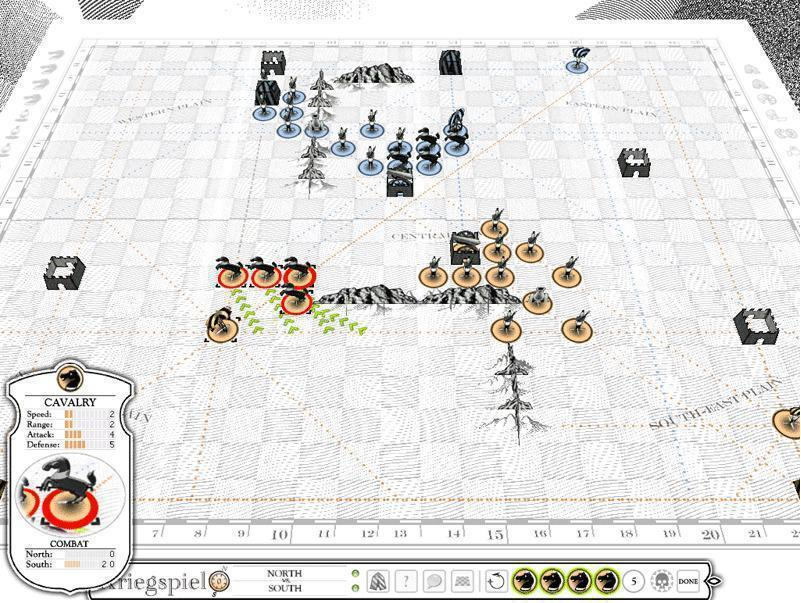
\includegraphics[scale=0.5]{data/kriegspiel.jpeg}
\caption{Jeu \textit{Kriegsspiel} : jeu de pions complexe développé par l'armée du royaume de Prusse au XIXe siècle pour enseigner les tactiques de combat aux officiers, adapte aussi dans des versions plus modernes \cite{livermore1879american}}
\end{figure}

Par exemple, Nous avons trouvé un jeu similaire à notre projet : \textit{Kriegsspiel}, un des plus anciens jeux de guerre , datant du XIXème siècle, initialement créé par des généraux Prussiens pour former leurs officiers.

\begin{figure}[H]
\centering
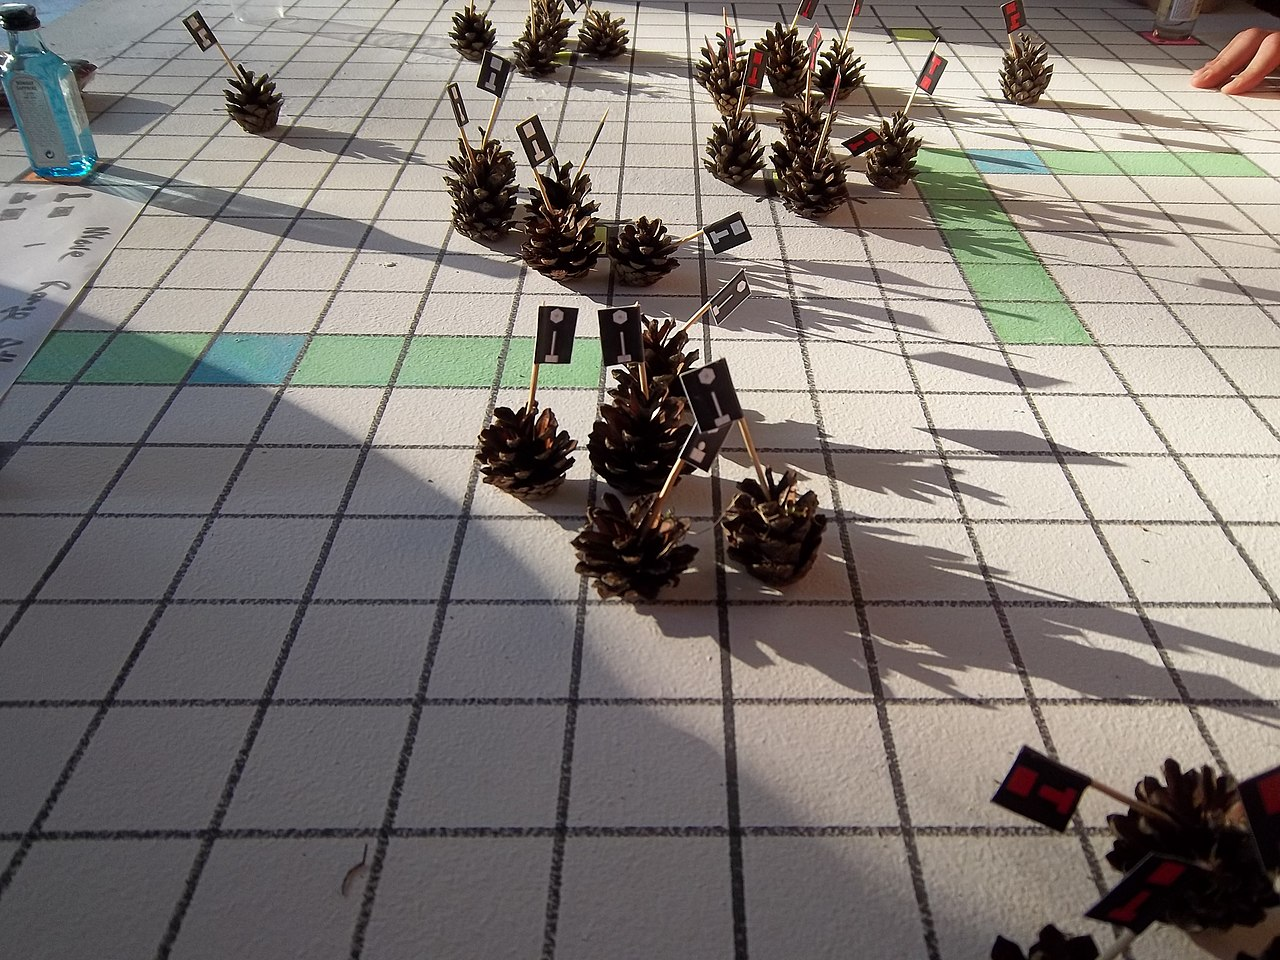
\includegraphics[scale=0.2]{data/Cavalry_at_dusk,.jpg}
\caption{\textit{Le Jeu de la guerre (War Game)} : Plateau du jeu}.
\end{figure}

Le Jeu de la Guerre \cite{frwiki:189457170} est un essai stratégique de Guy Debord et Alice Becker-Ho édité en 1987.
C'est un jeu qui se joue sur un plateau de 25x20. Contrairement à Desert Fox le plateau est en carré. La ressemblance avec Desert Fox est la formation d'unité (infanterie, cavalerie, artillerie).
